% !TeX program = pdflatex
% !TeX spellcheck = en_US
\documentclass[12pt,a4paper]{article}

%----------------------------------
% Packages
%----------------------------------
\usepackage[utf8]{inputenc}
\usepackage{graphicx}
\usepackage{geometry}
\usepackage{setspace}
\usepackage{hyperref}
\usepackage{caption}
\usepackage{booktabs}
\usepackage{float}
\usepackage{amsmath}

%----------------------------------
% Page setup
%----------------------------------
\geometry{a4paper, margin=1in}
\setstretch{1.5}
\setcounter{tocdepth}{3} % Ensures sub-sub-sections appear in the Table of Contents

\begin{document}
	
	%----------------------------------
	% Title Page 
	%----------------------------------
	\begin{titlepage}
		\begin{center}
			\vspace*{0.1cm}
			% Uncomment the line below and ensure 'mec_logo.png' is in the same folder
			
\includegraphics[width=3cm]{mec_logo.png}\\[0.25cm]
			{\Large \textbf{Model Engineering College, Thrikkakara}}\\[1pt]
			{\large Department of Electronics Engineering}\\[1pt]
			\vspace{0.5cm}
			{\huge \textbf{PROJECT REPORT}}\\[0.5cm]
			{\Large \textbf{on}}\\[0.5cm]
			{\LARGE \textbf{ Morse Code Trainer }}\\[1cm]
			{\Large Submitted by}\\[0.25cm]
			{\large \textbf{Francisca Thankachan (Roll No: 28)}\\
				\textbf{Jacob Saji (Roll No: 30)}\\
				\textbf{Jishnu Prashanth (Roll No: 32)}}\\[1 cm]
			{\large 4th Semester, Academic Year 2025–26}\\[0.2cm] 
			{\large B Tech (Electronics \& Commn Engineering)}\\[0.2cm]
			{\large \textbf{Signals and Systems}}\\[0.2cm]
			\vfill
			{\large \textbf{Department of Electronics and Communication Engineering}}\\[1pt]
			{\large Model Engineering College, Thrikkakara}\\[1pt]
			{\large (Affiliated to APJ Abdul Kalam Kerala Technological University)}\\[0.2cm]
			\vspace{0.2cm}
			\rule{0.9\textwidth}{0.4pt}\\[3pt]
			{\small \today}
		\end{center}
	\end{titlepage}
	\clearpage
	
	%----------------------------------
	% Front Matter
	%----------------------------------
	\pagenumbering{roman}
	
	% 1. TABLE OF CONTENTS FIRST
	\tableofcontents
	\clearpage
	
	% 2. LIST OF FIGURES (Makes the index highly detailed)
	\addcontentsline{toc}{section}{List of Figures}
	\listoffigures
	\clearpage
	
	% 3. ABSTRACT SECOND
	\section*{Abstract}
	\addcontentsline{toc}{section}{Abstract}
	The design and implementation of a hardware-based signal processing system that can decode human touch inputs into discrete alphanumeric text are presented in this project. The system uses real-time time-domain analysis to categorize signal pulse widths by treating user input as a continuous-time binary signal. The system effectively filters high-frequency mechanical noise (denouncing) and uses strict temporal threshold to distinguish between Morse code "dots" and "dashes" using an ESP32 micro controller, a capacitive touch sensor, and visual output modules. A look-up table is used to map the decoded discrete sequence, which is then shown on an LCD to illustrate a real-world use of dynamic, causal system design.
	\clearpage
	
	%----------------------------------
	% Main Content
	%----------------------------------
	\pagenumbering{arabic}
	
	\section{Introduction}
	While alternative communication systems frequently need to decode intricate temporal patterns from a single input channel, traditional data entry relies on multi-key interfaces. This project's main goal is to create an embedded system that connects discrete digital logic with continuous physical actions.This project provides a real-world application of basic signal processing concepts by using Morse code, a standard that is solely based on pulse-width modulation. The system is intended to obtain an aperiodic binary signal, sample it into a discrete-time array, and then use dynamic memory to convert unstructured temporal lengths into text that is readable by humans.
	
	\section{Block Diagram \& Component Specifications}
	\subsection{Block Diagram}
	% To insert your diagram, uncomment the block below and replace 'block_diagram.png' with your image file name
	\begin{figure}[H]
		\centering
		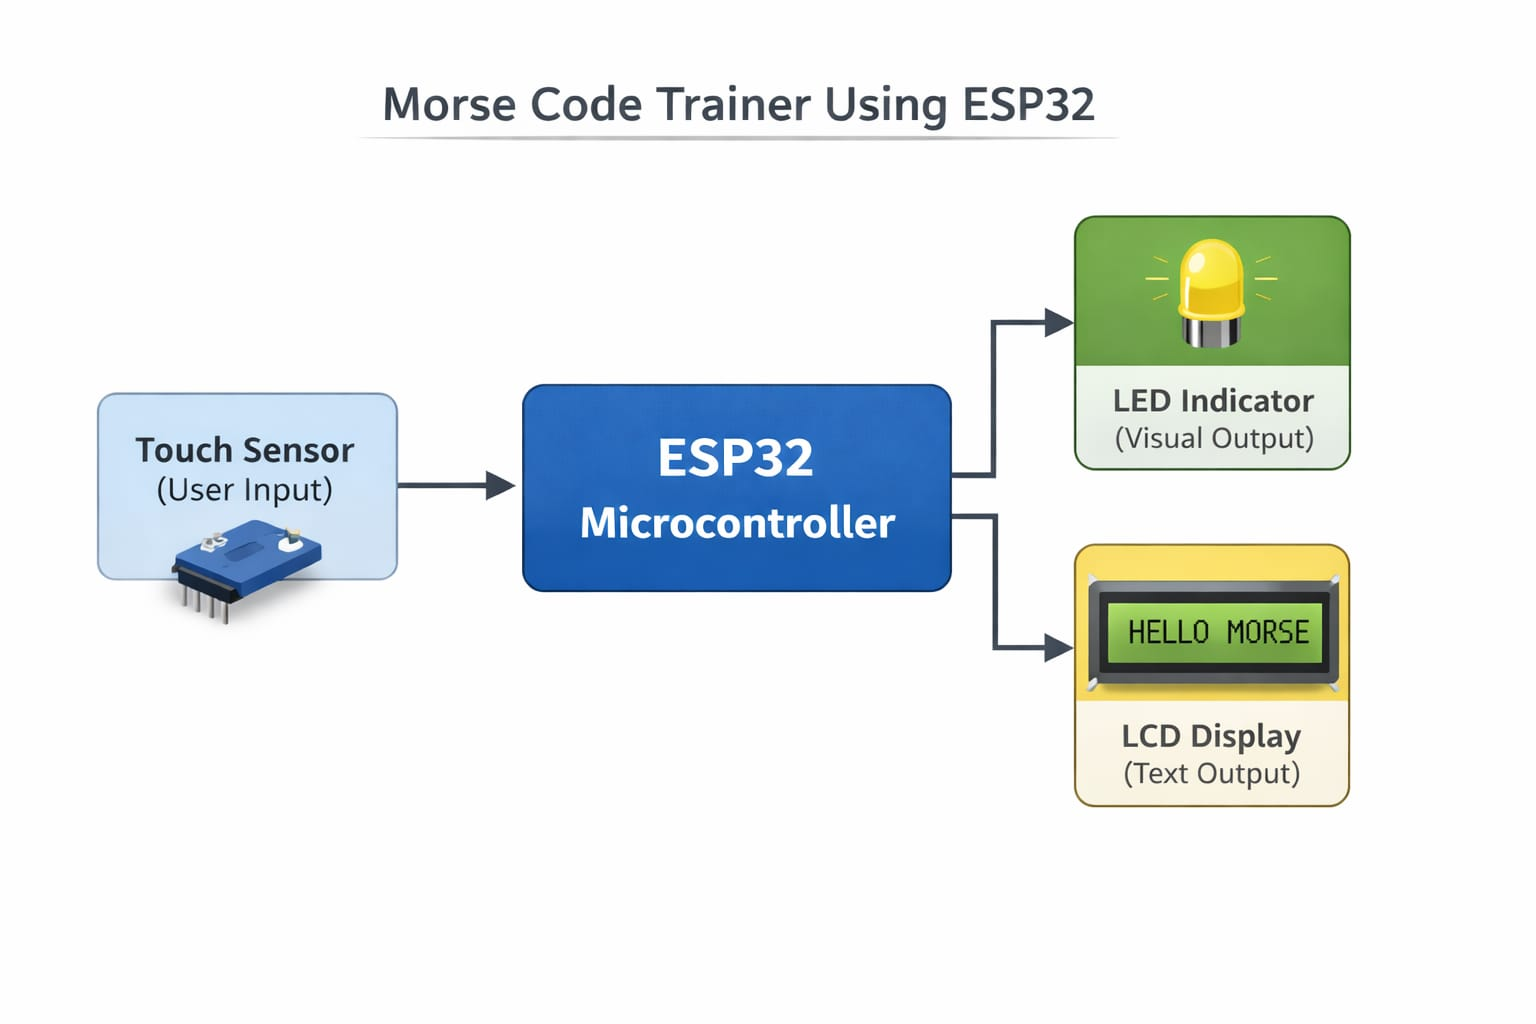
\includegraphics[width=0.8\textwidth]{BlockDiagram.jpg}
		\caption{System block diagram illustrating the flow from the continuous-time sensor input $x(t)$, through the ESP32 processing logic, to the discrete alphanumeric output $y[n]$ on the LCD.}
		\label{fig:block_diagram}
	\end{figure}
	
	
	\subsection{Component Specifications}
	\begin{itemize}
		\item \textbf{Microcontroller: ESP32-WROOM-32 38Pin Development Board WiFi+Bluetooth Ultra-Low Power Consumption Dual Core}
		\addcontentsline{toc}{subsubsection}{Microcontroller: ESP32-WROOM-32}
		\begin{figure}[H]
			\centering
			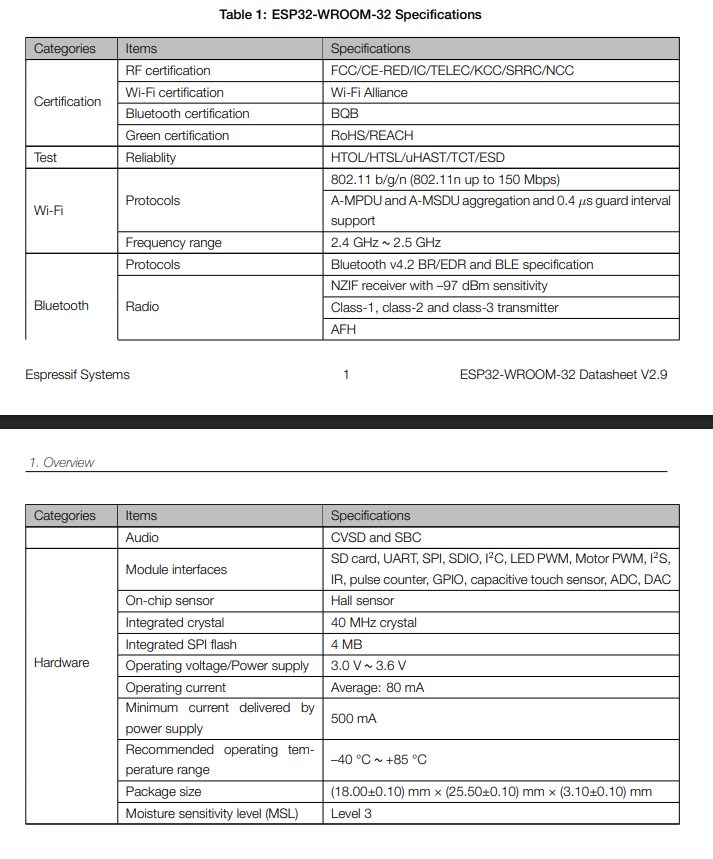
\includegraphics[width=0.8\textwidth]{ESP_SPEC.png}
			\caption{Technical specifications of the ESP32 Microcontroller}
			\label{fig:esp32_specs}
		\end{figure}
		\begin{figure}[H]
			\centering
			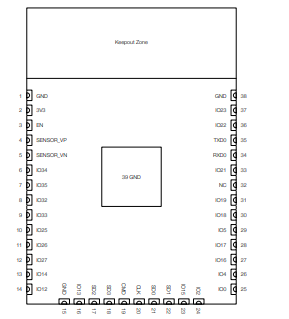
\includegraphics[width=0.8\textwidth]{PinLayout.png}
			\caption{Pin layout of ESP32-WROOM-32}
			\label{fig:esp32_specs}
		\end{figure}
		\begin{figure}[H]
			\centering
			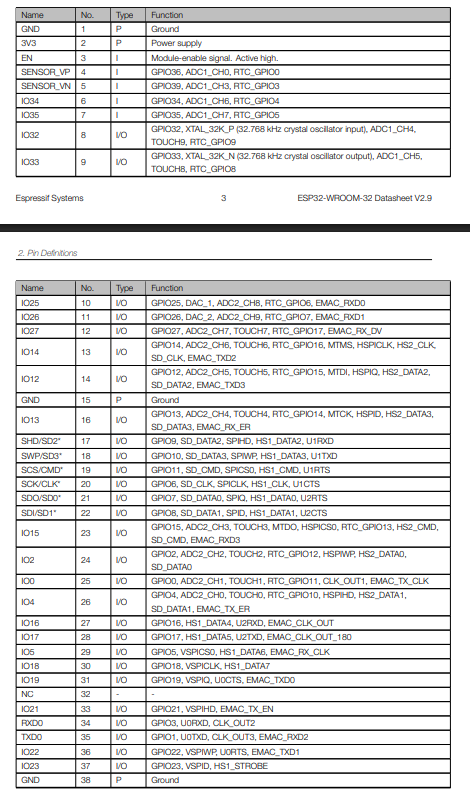
\includegraphics[width=0.8\textwidth]{pindis.png}
			\caption{Pin description of ESP32-WROOM-32}
			\label{fig:esp32_specs}
		\end{figure}
		
		\item \textbf{Input : TTP223 Capacitive Touch Sensor}
		\addcontentsline{toc}{subsubsection}{Input: TTP223 Capacitive Touch Sensor}
		\begin{figure}[H]
			\centering
			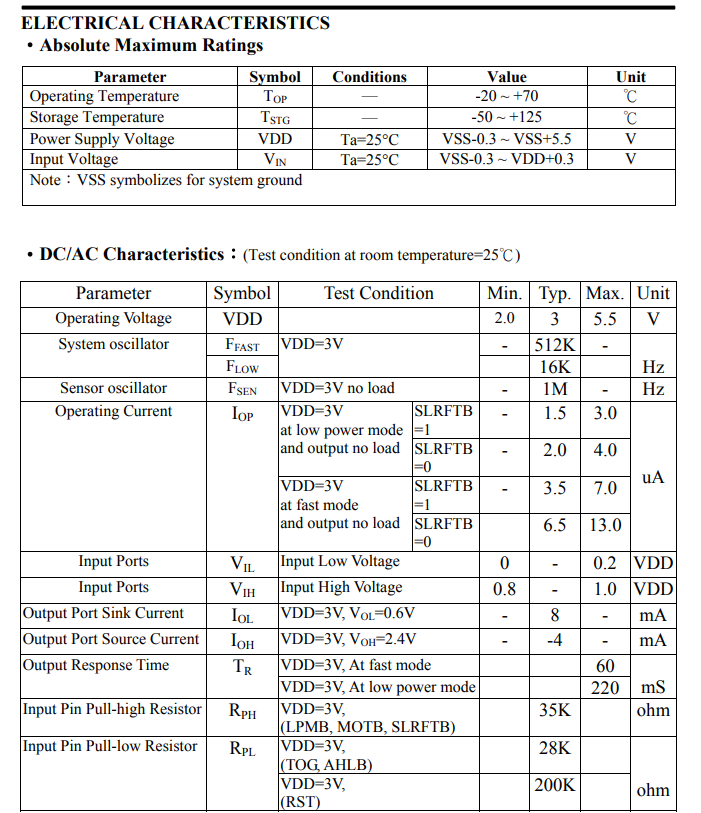
\includegraphics[width=0.8\textwidth]{touch.png}
			\caption{Electrical specifications of TTP223}
			\label{fig:esp32_specs}
		\end{figure}
		
		\item \textbf{ Output: LCD1602 Parallel LCD Display with IIC/I2C interface}
		\addcontentsline{toc}{subsubsection}{Output 1: LCD1602 Parallel LCD Display}
		\begin{figure}[H]
			\centering
			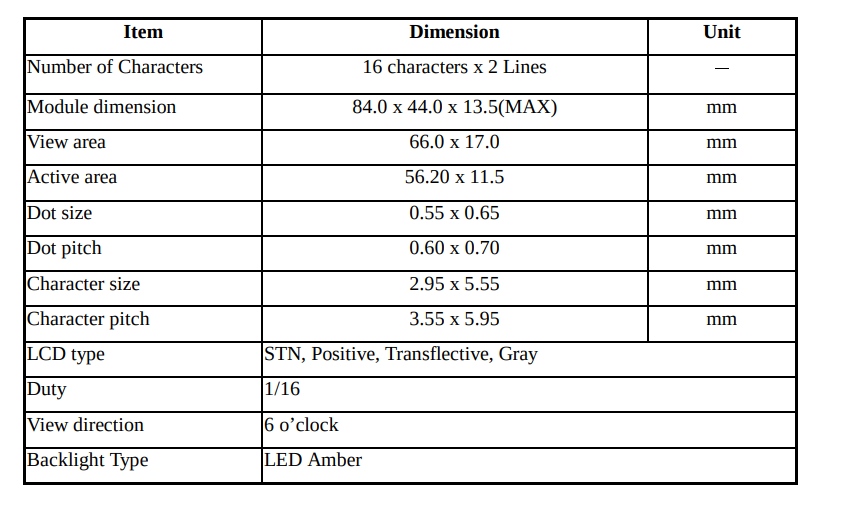
\includegraphics[width=0.8\textwidth]{lcdgs.png}
			\caption{General specs of 16X2 LCD display }
			\label{fig:esp32_specs}
		\end{figure}
		\begin{figure}[H]
			\centering
			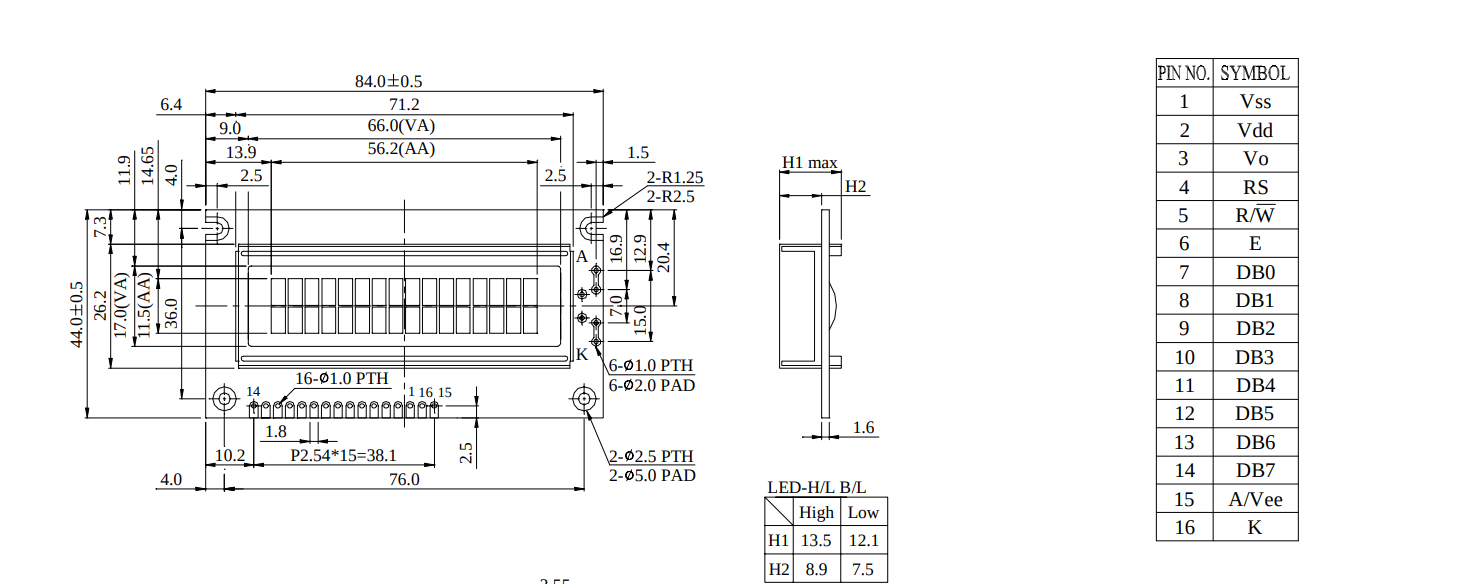
\includegraphics[width=0.8\textwidth]{LCDpin.png}
			\caption{Pin diagram of 16X2 LCD display}
			\label{fig:esp32_specs}
		\end{figure}
		\begin{figure}[H]
			\centering
			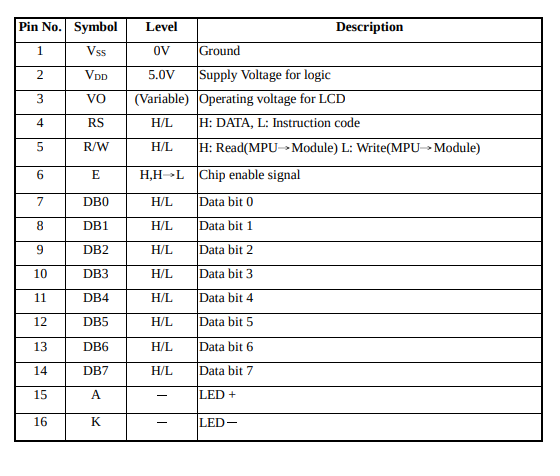
\includegraphics[width=0.8\textwidth]{lcdf.png}
			\caption{Pin functions of 16X2 LCD display}
			\label{fig:esp32_specs}
		\end{figure}
		\begin{figure}[H]
			\centering
			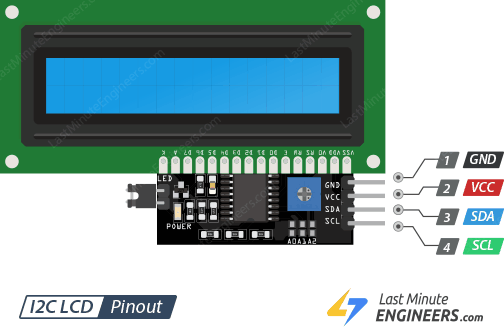
\includegraphics[width=0.8\textwidth]{I2C-LCD-Display-Pinout.png}
			\caption{Pin diagram of 16X2 LCD display with I2C module}
			\label{fig:esp32_specs}
		\end{figure}
		
		\item \textbf{ Output 2: 5mm Round RGB LED}
		\addcontentsline{toc}{subsubsection}{Output 2: 5mm Round RGB LED}
		\begin{figure}[H]
			\centering
			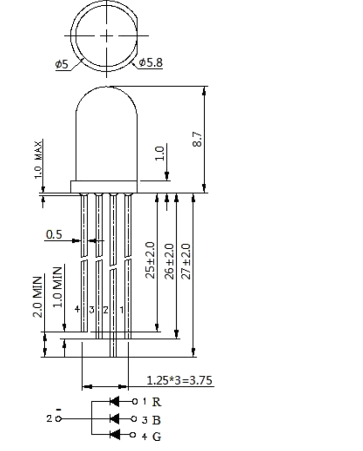
\includegraphics[width=0.8\textwidth]{Screenshot from 2026-03-25 21-09-42.png}
			\caption{Pin diagram of 5mm Round RGB LED}
			\label{fig:esp32_specs}
		\end{figure}
		\begin{figure}[H]
			\centering
			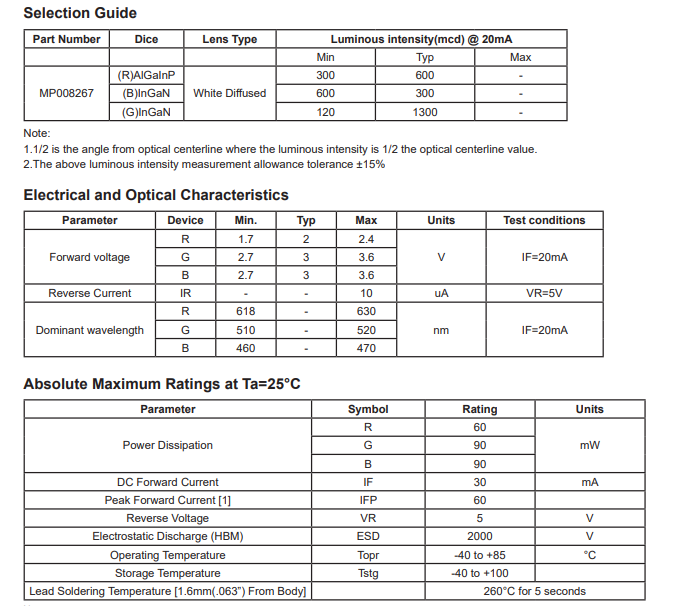
\includegraphics[width=0.8\textwidth]{Screenshot from 2026-03-25 21-11-23.png}
			\caption{Specifications of 5mm Round RGB LED}
			\label{fig:esp32_specs}
		\end{figure}
	\end{itemize}
	
	\section{Working Methodology}
	The system processes the user's touch input in four simple, logical steps to figure out which letter was typed:
	
	\begin{enumerate}
		\item \textbf{Detecting the Touch :} 
		The ESP32 microcontroller constantly watches the touch sensor. The moment a user places their finger on the sensor, the system starts a digital stopwatch to record the exact start time.
		\addcontentsline{toc}{subsubsection}{1. Detecting the Touch}
		
		\item \textbf{Filtering out Accidental Bumps :} 
		When the user lifts their finger, the stopwatch stops, giving us the total time of the touch. If the touch lasted for less than 50 milliseconds, the system assumes it was just an accidental brush or a brief electrical glitch. It completely ignores these micro-touches to prevent mistakes.
		\addcontentsline{toc}{subsubsection}{2. Filtering out Accidental Bumps}
		
		\item \textbf{Figuring out Dot vs. Dash :} 
		If the touch was valid, the system looks at exactly how long the user held their finger down to classify it:
		\begin{itemize}
			\item \textbf{A Quick Tap (Dot):} If the touch lasted between 50 and 250 milliseconds, it is recorded as a `Dot'. The system immediately flashes a Green LED to show the user it registered a dot.
			\item \textbf{A Long Hold (Dash):} If the touch lasted longer than 600 milliseconds, it is recorded as a `Dash'. The system flashes a Blue LED to show it registered a dash.
		\end{itemize}
		\addcontentsline{toc}{subsubsection}{3. Figuring out Dot vs. Dash}
		
		\item \textbf{Finding the Letter :} 
		The system remembers the sequence of dots and dashes as you type them (for example, saving ``Dot-Dash'' for the letter 'A'). It then waits to see what the user does next. If the user leaves their finger off the sensor for more than 1 full second, the system knows the sequence is finished. It checks its built-in dictionary (Look-Up Table) to find which alphabet letter matches the dots and dashes, prints that letter on the LCD screen, and gets ready for the next word.
		\addcontentsline{toc}{subsubsection}{4. Finding the Letter}
	\end{enumerate}
	
	\section{Output \& Waveform Analysis}
	\subsection{Physical Output}
	% To insert your photo, uncomment the block below and replace 'hardware_setup.jpg' with your image file name
	\begin{figure}[H]
		\centering
		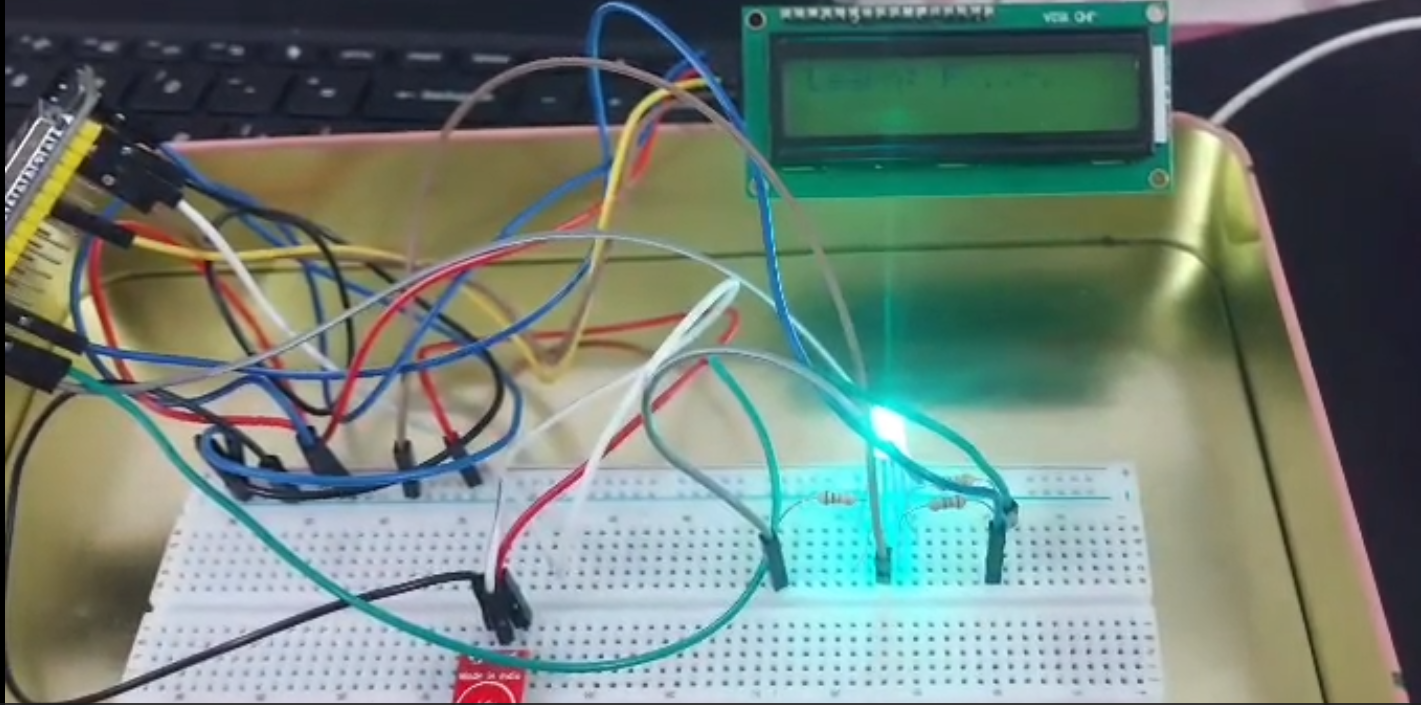
\includegraphics[width=0.6\textwidth]{Screenshot from 2026-03-25 21-19-30.png}
		\caption{Physical breadboard setup displaying text on the LCD}
		\label{fig:hardware}
	\end{figure}
	
	
	\section{Conclusion}
	The project successfully realized a hardware-based signal decoder capable of translating human interaction into digital text. By implementing software-based debouncing and time-domain thresholding, the system achieved a highly accurate discrimination between transient noise, short impulses, and long step signals. This project practically verified that a dynamic, causal, and non-linear system can reliably map continuous physical actions into structured, discrete information using affordable embedded components.
	
	\section{Future Scope}
	While the current system is highly functional, several improvements can be made for broader application:
	\begin{itemize}
		\item \textbf{Audio Feedback Integration:} Adding a piezoelectric buzzer driven by a PWM signal to provide traditional auditory Morse code feedback alongside the visual LED.
		\item \textbf{Adaptive Thresholding:} Implementing a machine-learning algorithm to track the user's average typing speed over time and dynamically adjust the 250ms and 600ms thresholds, allowing the system to adapt to fast or slow typists automatically.
		\item \textbf{Wireless Transmission:} Utilizing the ESP32's native Wi-Fi or Bluetooth capabilities to transmit the decoded text to a smartphone app or remote server in real-time.
	\end{itemize}
	
\end{document}